\documentclass[margin=5mm]{standalone}
\usepackage{tikz}
\usetikzlibrary{positioning,arrows.meta}
\usetikzlibrary{calc}
\usetikzlibrary{shadows.blur}
\usetikzlibrary{backgrounds}
\usetikzlibrary{patterns}

% Communication system block diagram
\begin{document}

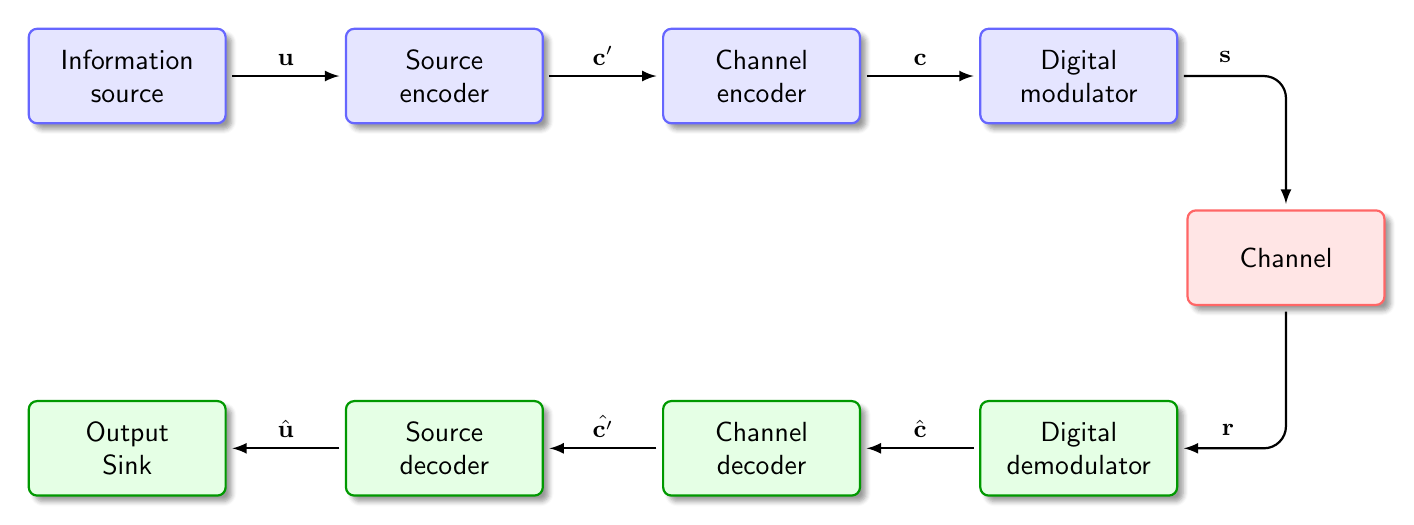
\begin{tikzpicture}[
    % Transmitter
    tx block/.style={
        draw=blue!60,
        fill=blue!10,
        thick,
        rounded corners=3pt,
        minimum width=2.5cm,
        minimum height=1.2cm,
        align=center,
        blur shadow={shadow blur steps=5},
        font=\sffamily
    },
    % Receiver
    rx block/.style={
        draw=green!60!black,
        fill=green!10,
        thick,
        rounded corners=3pt,
        minimum width=2.5cm,
        minimum height=1.2cm,
        align=center,
        blur shadow={shadow blur steps=5},
        font=\sffamily
    },
    % Channel
    channel block/.style={
        draw=red!60,
        fill=red!10,
        thick,
        rounded corners=3pt,
        minimum width=2.5cm,
        minimum height=1.2cm,
        align=center,
        blur shadow={shadow blur steps=5},
        font=\sffamily
    },
    % Arrow
    arrow/.style={
        ->,
        >=latex,
        thick,
        shorten >=2pt,
        shorten <=2pt
    }
]

% Top row blocks (Transmitter chain)
\node[tx block] (source) {Information\\source};
\node[tx block, right=1.5cm of source] (sourceenc) {Source\\encoder};
\node[tx block, right=1.5cm of sourceenc] (channelenc) {Channel\\encoder};
\node[tx block, right=1.5cm of channelenc] (modulator) {Digital\\modulator};

% Channel block
\node[channel block] (channel) at ($(modulator)!0.5!(modulator.south east)+(2cm,-2cm)$) {Channel};

% Bottom row blocks (Receiver chain)
\node[rx block, below=3.5cm of modulator] (demodulator) {Digital\\demodulator};
\node[rx block, left=1.5cm of demodulator] (channeldec) {Channel\\decoder};
\node[rx block, left=1.5cm of channeldec] (sourcedec) {Source\\decoder};
\node[rx block, left=1.5cm of sourcedec] (output) {Output\\Sink};

% Decorative connection with signal notations
\begin{scope}[rounded corners=8pt]
    % Transmitter path
    \draw[arrow] (source) -- node[above, font=\small] {$\mathbf{u}$} (sourceenc);
    \draw[arrow] (sourceenc) -- node[above, font=\small] {$\mathbf{c}'$} (channelenc);
    \draw[arrow] (channelenc) -- node[above, font=\small] {$\mathbf{c}$} (modulator);
    \draw[arrow] (modulator) -- node[above right = 1pt and 4pt, font=\small] {$\mathbf{s}$} ($(modulator.east)+(0.5,0)$) -| node[right, font=\small] {} (channel);
    
    % Receiver path
    \draw[arrow] (channel) |- node[above left = 1pt and 15pt, font=\small] {$\mathbf{r}$} (demodulator);
    \draw[arrow] (demodulator) -- node[above, font=\small] {$\hat{\mathbf{c}}$} (channeldec);
    \draw[arrow] (channeldec) -- node[above, font=\small] {$\hat{\mathbf{c}'}$} (sourcedec);
    \draw[arrow] (sourcedec) -- node[above, font=\small] {$\hat{\mathbf{u}}$} (output);
\end{scope}

% % Caption
% \node[font=\small\sffamily, text=blue!60] at ($(source)+(0,-1cm)$) {Transmitter};
% \node[font=\small\sffamily, text=green!60!black] at ($(output)+(0,1cm)$) {Receiver};

% Background
\begin{scope}[on background layer]
    \fill[top color=blue!5,bottom color=green!5] 
        ($(source)+(-0.5,-0.5)$) rectangle ($(output)+(0.5,4.5)$);
\end{scope}

\end{tikzpicture}
\end{document}